\documentclass[journal]{IEEEtran}

%\usepackage[brazil]{babel}
%\usepackage[T1]{fontenc}

\usepackage{theorem}        %%Lo agregue yo <========================================
\usepackage{algorithmic}        %%Lo agregue yo <========================================

\setcounter{secnumdepth}{7}

\newtheorem{theorem}{Theorem}%[section]
%\newtheorem{acknowledgement}[theorem]{Acknowledgement}
%\newtheorem{algorithm}[theorem]{Algorithm}
%\newtheorem{axiom}[theorem]{Axiom}
%\newtheorem{case}[theorem]{Case}
%\newtheorem{claim}[theorem]{Claim}
%\newtheorem{conclusion}[theorem]{Conclusion}
%\newtheorem{condition}[theorem]{Condition}
%\newtheorem{conjecture}[theorem]{Conjecture}
%\newtheorem{criterion}[theorem]{Criterion}
%\newtheorem{exercise}[theorem]{Exercise}
%\newtheorem{notation}[theorem]{Notation}
%\newtheorem{problem}[theorem]{Problem}
%\newtheorem{proposition}[theorem]{Proposition}
%\newtheorem{remark}[theorem]{Remark}
%\newtheorem{solution}[theorem]{Solution}
%\newtheorem{summary}[theorem]{Summary}

\newtheorem{definition}[theorem]{Definition}
\newtheorem{example}[theorem]{Example}
\newtheorem{lemma}[theorem]{Lemma}
\newenvironment{proof}[1][Proof]{\textbf{#1.} }{\ \rule{0.5em}{0.5em}}
\newtheorem{corollary}[theorem]{Corollary}
\newenvironment{algorithm}[1][Algorithm]{\textbf{#1.} }{}

\usepackage{amssymb}
\usepackage{graphicx}
\usepackage{amsmath}
\usepackage{psfrag}

\usepackage{accents}
%\usepackage[none]{hyphenat}

\usepackage[usenames,dvipsnames,svgnames,table]{xcolor}

\hyphenation{bet-ween re-pre-sen-ting} %
\sloppy

\begin{document}

\title{Approximate Joint Entropy for $M$ Correlated Binary Sources }


\author{Fernando P. Rivera 
\thanks{Manuscript received XXXX XX, 2014; revised XXXXX XX, 2014.}
\thanks{---------- ---------- ---------- ---------- ---------- ---------- ---------- ---------- ---------- ---------- ---------- }%%%%Fernando P. Rivera is with Department of Communications, State University of Campinas, Campinas, SP, Brazil. Email:fpujaico@decom.fee.unicamp.br. }
\thanks{---------- ---------- ---------- ---------- ---------- ---------- ---------- ---------- ---------- ---------- ---------- }}%%%%Jaime Portugheis   is with Faculty of Technology       , State University of Campinas, Limeira , SP, Brazil. Email:jaime@ft.unicamp.br  .}}

\markboth{IEEE Communications Letters,~Vol.~X,
No.~XX,~XXXXX~XXX}{Shell \MakeLowercase{\textit{et al.}}: Bare
Demo of IEEEtran.cls for Journals}

% make the title area
\maketitle
%%%%%%%\IEEEpeerreviewmaketitle


\begin{abstract}
This paper proposes a method for to get an approximation of the joint entropy
of $M$ correlated binary sources; the approximation gets a linear calculation complexity 
in relation to the number of sources. 
Here, it is used a correlating model with a common
binary source that through $M$ binary symmetric channels in parallel
to obtain  the $M$ correlated binary sources. 

\end{abstract}

%\begin{keywords}
%Multiple correlated sources, large scale sensor networks, joint entropy.
%\end{keywords}

\IEEEpeerreviewmaketitle
%%%%%%%%%%%%%%%%%%%%%%%%%%%%%%%%%%%%%%%%%%%%%%%%%%%%%%%%%%%%%%%%%%%%%%%%%%%%%%%%%%%%%%%
%%%%%%%%%%%%%%%%%%%%%%%%%%%%%%%%%%%%%%%%%%%%%%%%%%%%%%%%%%%%%%%%%%%%%%%%%%%%%%%%%%%%%%%
%%%%%%%%%%%%%%%%%%%%%%%%%%%%%%%%%%%%%%%%%%%%%%%%%%%%%%%%%%%%%%%%%%%%%%%%%%%%%%%%%%%%%%%
\section{Introduction}
\label{sec:Intro}
 
 
This paper is organized as follows. The model system and some definitions 
used in this work are presented in Section \ref{sec:SystemModel}, the current method for to get the joint entropy is presented in Section \ref{sec:Joint}, in this line a new method for to get
the joint entropy is described in Section \ref{sec:NewJoint}. 
The test of the for to get the joint entropy is presented in Section \ref{sec:Test}
Some demonstrations
need for to solve the last sections are presented in
Section \ref{sec:Appendix} and Section \ref{sec:Conclusions} concludes the paper 
with some final remarks.

%%%%%%%%%%%%%%%%%%%%%%%%%%%%%%%%%%%%%%%%%%%%%%%%%%%%%%%%%%%%%%%%%%%%%%%%%%%%%%
%%%%%%%%%%%%%%%%%%%%%%%%%%%%%%%%%%%%%%%%%%%%%%%%%%%%%%%%%%%%%%%%%%%%%%%%%%%%%%
%%%%%%%%%%%%%%%%%%%%%%%%%%%%%%%%%%%%%%%%%%%%%%%%%%%%%%%%%%%%%%%%%%%%%%%%%%%%%%
\section{System Model and Definitions} \label{sec:SystemModel}

The Fig. \ref{fig:model} show $M$ correlated binary sources $U_m$, $1 \leq m \leq M| i \in \mathbb{N}$.
This sources

\label{sec:SystemModel}
\begin{figure}[!h]
  \centering
    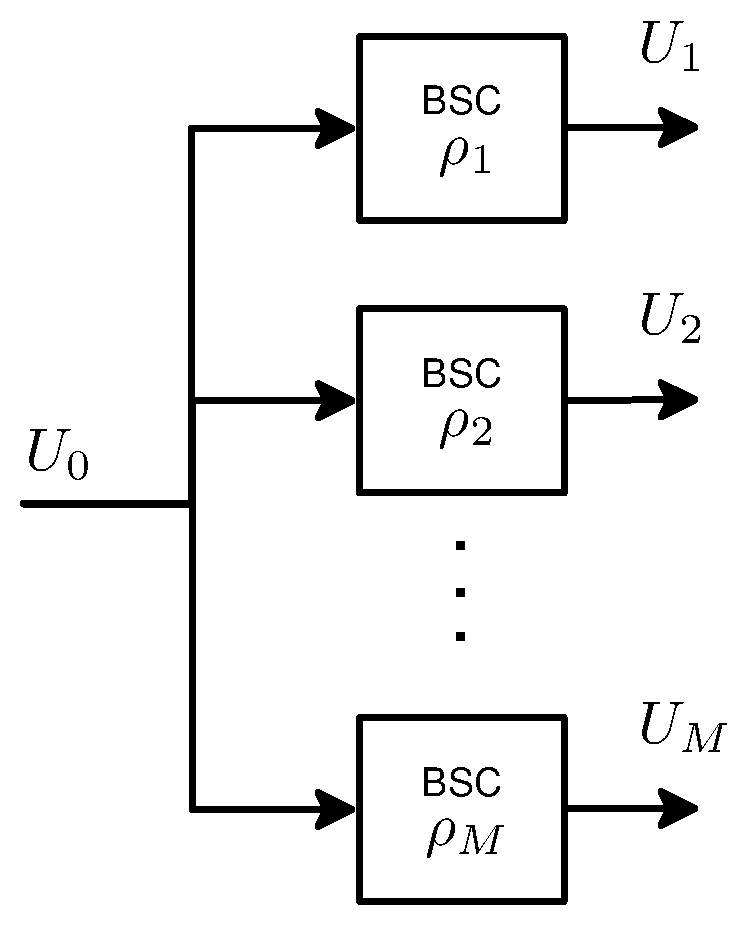
\includegraphics[width=0.8\columnwidth]{sources.eps}
  \caption{$M$ correlated binary sources.}
    \label{fig:model}
\end{figure}

%%%%%%%%%%%%%%%%%%%%%%%%%%%%%%%%%%%%%%%%%%%%%%%%%%%%%%%%%%%%%%%%%%%%%%%%%%%%%%
%%%%%%%%%%%%%%%%%%%%%%%%%%%%%%%%%%%%%%%%%%%%%%%%%%%%%%%%%%%%%%%%%%%%%%%%%%%%%%
%%%%%%%%%%%%%%%%%%%%%%%%%%%%%%%%%%%%%%%%%%%%%%%%%%%%%%%%%%%%%%%%%%%%%%%%%%%%%%
\section{Joint entropy in correlated } \label{sec:Joint}

\subsection{General formulation of joint entropy}
\subsection{Specific formulation of joint entropy when $\rho_i=\rho$}
%%%%%%%%%%%%%%%%%%%%%%%%%%%%%%%%%%%%%%%%%%%%%%%%%%%%%%%%%%%%%%%%%%%%%%%%%%%%%%
%%%%%%%%%%%%%%%%%%%%%%%%%%%%%%%%%%%%%%%%%%%%%%%%%%%%%%%%%%%%%%%%%%%%%%%%%%%%%%
%%%%%%%%%%%%%%%%%%%%%%%%%%%%%%%%%%%%%%%%%%%%%%%%%%%%%%%%%%%%%%%%%%%%%%%%%%%%%%
\section{Proposed joint entropy calculus } \label{sec:NewJoint}

%%%%%%%%%%%%%%%%%%%%%%%%%%%%%%%%%%%%%%%%%%%%%%%%%%%%%%%%%%%%%%%%%%%%%%%%%%%%%%
%%%%%%%%%%%%%%%%%%%%%%%%%%%%%%%%%%%%%%%%%%%%%%%%%%%%%%%%%%%%%%%%%%%%%%%%%%%%%%
%%%%%%%%%%%%%%%%%%%%%%%%%%%%%%%%%%%%%%%%%%%%%%%%%%%%%%%%%%%%%%%%%%%%%%%%%%%%%%
\section{Numerical analyses } \label{sec:Test}

%%%%%%%%%%%%%%%%%%%%%%%%%%%%%%%%%%%%%%%%%%%%%%%%%%%%%%%%%%%%%%%%%%%%%%%%%%%%%%
%%%%%%%%%%%%%%%%%%%%%%%%%%%%%%%%%%%%%%%%%%%%%%%%%%%%%%%%%%%%%%%%%%%%%%%%%%%%%%
%%%%%%%%%%%%%%%%%%%%%%%%%%%%%%%%%%%%%%%%%%%%%%%%%%%%%%%%%%%%%%%%%%%%%%%%%%%%%%
\section{Demonstrations } \label{sec:Appendix}

%%%%%%%%%%%%%%%%%%%%%%%%%%%%%%%%%%%%%%%%%%%%%%%%%%%%%%%%%%%%%%%%%%%%%%%%%%%%%%
%%%%%%%%%%%%%%%%%%%%%%%%%%%%%%%%%%%%%%%%%%%%%%%%%%%%%%%%%%%%%%%%%%%%%%%%%%%%%%
%%%%%%%%%%%%%%%%%%%%%%%%%%%%%%%%%%%%%%%%%%%%%%%%%%%%%%%%%%%%%%%%%%%%%%%%%%%%%%
\section{Final Remarks and Conclusions} 
\label{sec:Conclusions}
In this letter, we considered joint source-channel coding of correlated
sources transmitted over orthogonal

%%%%%%%%%%%%%%%%%%%%%%%%%%%%%%%%%%%%%%%%%%%%%%%%%%%%%%%%%%%%%%%%%%%%%%%%%%%%%%
%%%%%%%%%%%%%%%%%%%%%%%%%%%%%%%%%%%%%%%%%%%%%%%%%%%%%%%%%%%%%%%%%%%%%%%%%%%%%%
%%%%%%%%%%%%%%%%%%%%%%%%%%%%%%%%%%%%%%%%%%%%%%%%%%%%%%%%%%%%%%%%%%%%%%%%%%%%%%
%%%%%%%%%%%%%%%%%%%%%%%%%%%%%%%%%%%%%%%%%%%%%%%%%%%%%%%%%%%%%%%%%%%%%%%%%%%%%%
\section*{Acknowledgment}

%%%%%%%%%%%%%%%%%%%%%%%%%%%%%%%%%%%%%%%%%%%%%%%%%%%%%%%%%%%%%%%%%%%%%%%%%%%%%%
%%%%%%%%%%%%%%%%%%%%%%%%%%%%%%%%%%%%%%%%%%%%%%%%%%%%%%%%%%%%%%%%%%%%%%%%%%%%%%
%%%%%%%%%%%%%%%%%%%%%%%%%%%%%%%%%%%%%%%%%%%%%%%%%%%%%%%%%%%%%%%%%%%%%%%%%%%%%%
%\appendix
\section{Appendix} \label{sec:Appendix}

%%%%%%%%%%%%%%%%%%%%%%%%%%%%%%%%%%%%%%%%%%%%%%%%%%%%%%%%%%%%%%%%%%%%%%%%%%%%%%
%%%%%%%%%%%%%%%%%%%%%%%%%%%%%%%%%%%%%%%%%%%%%%%%%%%%%%%%%%%%%%%%%%%%%%%%%%%%%%
%%%%%%%%%%%%%%%%%%%%%%%%%%%%%%%%%%%%%%%%%%%%%%%%%%%%%%%%%%%%%%%%%%%%%%%%%%%%%%
\begin{thebibliography}{99}

\bibitem{fernando} Pujaico, F.; Portugheis, J.,
``Optimal Rate for Joint Source-Channel Coding of Correlated Sources Over 
Orthogonal Channels,'' Communications Letters, 2014.

\bibitem{ceobinary1} Haghighat, J.; Behroozi, Hamid; Plant, D.V., 
``Iterative joint decoding for sensor networks with binary CEO model,'' 
Signal Processing Advances in Wireless Communications, 2008. SPAWC 2008. 
IEEE 9th Workshop on , vol., no., pp.41,45, 6-9 July 2008.

\end{thebibliography}

\end{document}

